% !TeX spellcheck = es_ES
\chapter{Palabras nuevas}


% Intro {{{

En el capítulo anterior, se mencionó que el algoritmo toma como  idioma
dominante a aquel que transmite palabras hacia los demás y que estas perduran en los receptores al menos dos años.  El movimiento de palabras, es una característica que puede proporcionar información sobre la influencia entre los idiomas, sin embargo  puede resultar ambiguo decir que algo es más o menos influyente, además  no existe en la literatura un método que mida la influencia.

%El empleo de estás características puede proporcionar información acerca de la influencia que ejercen los idiomas,  sin  embargo, establecer un método que brinde un resultado al cual ligar la expresión influencia  no es sencillo, no existe en la literatura tal proceso, además puede ser ambiguo decir que algo es más o menos influyente sin un valor que lo respalde


%Al momento, en la literatura no existe una serie de pasos a seguir cuyo resultado final sea una cantidad que mida la influencia. Para llegar a esta resolución se requieren establecer nuevas condiciones en la base de datos, y a partir de ellas trazar posibles caminos que lleven a relaciones y resultados  con los cuales satisfacer una interpretación de la influencia

%\fxnote{ah? Otra palabra que no cuadra para nada\ldots}, 
%\fxnote{No  entiendo la ultima frase. Ten cuidado con los cambios. Siento que lo intentas hacer un poco rococo y elegante, pero por tratar, pierdes precision. Creo qeu lo mas importante  en textos cientificos es ser preciso, ordenado y conciso.}.


% \fxnote{division? No entendi\ldots}
% \fxwarning{deje comentado el texto donde me dejaste la nota y lo cmabie por el siguiente} 
% 
% \fxwarning{Ya trate de ser más conciso en lo que quiero decir, corregi todo el parrafo}
% 



 

%El llegar a esta conclusión requiere el establecer condiciones y características en los elementos para poder llegar a un resultado que satisfaga una interpretación de la influencia. 


% \fxnote{Ya no entiendo que quieres lograr con el siguietne parrafo. No se cual es el mensaje principal. De nuevo ``teñir un panorama'' no me suena correcto. Hablemos de la estructura de un parrafo y creo que tocara iterar de neuvo!!! Argh.}
% \fxwarning{ya Corregí todo el ,  dejo comentado el parrafo viejo}

%Aludiendo al capítulo  anterior, el tratamiento de la base de datos brinda información de los orígenes, los receptores y las palabras que migran de un lado a otro; comenzando con estos elementos, un primer paso es identificar los tiempos donde ocurren las migraciones. Antes de comprometer completamente al tiempo, es conveniente hacer una clasificación dentro de los propios préstamos para teñir un panorama más claro con el cual trabajar. 

Un primer paso para llegar a un valor que cuantifique a la influencia, es al estudiar los tiempos donde ocurren las migraciones, para encontrar relaciones entre dichos tiempos y las palabras involucradas en el movimiento. Antes de
profundizar en esta idea, es conveniente realizar una clasificación dentro los
préstamos, trabajar sobre ella y poder llegar a la cuantificación. 

Si se tiene una pareja de idioma origen \textit{A} e idioma receptor
\textit{B},  dentro de los préstamos de \textit{A} en \textit{B} se definen
como  \textbf{préstamos nuevos} a las  palabras que aparecen por primera vez en
las más usadas del idioma \textit{B}. Esta definición permite ordenar a los
préstamos nuevos por cada pareja de origen y receptor, y dentro  de este
ordenamiento, una segunda organización  por el año en el cual aparecieron. 



Dada la nueva clasificación, se determinaron tres posibilidades con las cuales
interpretar la influencia de un idioma sobre otro. 

\begin{enumerate}
	\label{proceso.nuevos}
	
\item Contar por cada año los préstamos nuevos de origen \textit{A} que están presentes en los diferentes receptores. Esto muestra en cuales idiomas \textit{A} ha sido influyente. 

\item Contar cuántos préstamos nuevos de diferentes orígenes están presentes en cada año, si se toma a \textit{A} como receptor. Con ello se obtienen los idiomas que han influenciado a \textit{A}

%Intercambiando a \textit{A}  como el idioma receptor, y contando cuántos préstamos nuevos de diferentes orígenes están presentes en cada año, obteniendo los idiomas que han influenciado a \textit{A}.  



\item Tomar fijos dos idiomas \textit{A} y \textit{B}, y contar cuántos préstamos nuevos de \textit{A} están en \textit{B} así como cuantos de \textit{B} lo están en \textit{A}.  Así se obtiene cómo ha sido la influencia entre \textit{A} y \textit{B}.

%contabilizando cuántos préstamos nuevos por año se encuentran al tomar a  \textit{A} como origen y a \textit{B} como receptor,  una vez hecho esto,  repetir el conteo intercambiando a \textit{B} como el origen y a \textit{A} como el receptor. Obteniendo las épocas donde alguno de ellos tuvo más del punto uno o del dos. 


\end{enumerate}


% }}}
\section{Eventos que ayudan a las migraciones} % {{{

Una parte complementaria de interpretar a la influencia es al reconocer las causas que originan las migraciones. Por ejemplo, sucesos como la globalización y el acceso al desarrollo tecnológico a finales de 1980 y principios de 1990, propiciaron la migración  de términos como \textit{internet}, \textit{computadora}, \textit{web}, \textit{email} o \textit{software}; el movimiento de este grupo de palabras se puede interpretar como una consecuencia del desarrollo e impacto de ambos eventos. 

Las causas que originan las migraciones, serán identificables a partir del significado de los préstamos involucrados en un año de migración. De acuerdo a \cite{mcgraw}, un  \textbf{campo semántico} es un conjunto de palabras asociadas que comparten parte de su significado. Entonces las palabras migrantes pueden estar relacionadas con un evento a partir de un campo semántico esto será identificable porque las migraciones ocurren en el mismo año (o en los años al rededor) donde el evento aconteció. 






%Una parte complementaria de interpretar la influencia es reconocer posibles causas que favorecen a las migraciones,  identificables por el tiempo donde ocurren, es decir, en un año de migración el significado de las palabras puede guardar alguna relación con un evento ocurrido durante el mismo año  (o en los años al rededor de él),  ya que las palabras migrantes pueden pertenecer a un mismo campo semántico relacionado al  evento. Por ejemplo, la globalización y el acceso al desarrollo tecnológico a finales de la década de 1980 y principios de 1990 propició la migración  de términos como \textit{internet}, \textit{computadora}, \textit{web}, \textit{email} o \textit{software}, mostrando a ambos ámbitos como propagadores del movimiento entre un origen y los distintos receptores. Al tratar con idiomas, se espera que en los eventos estén comprometidos países, personajes o comunidades que hablen o utilicen las lenguas involucradas. 












% }}}
\section{Préstamos nuevos entre idiomas durante el siglo XX } % {{{
\cpnote{naalisis
de palabras migrantes por pares de idiomas y tiempo, Prestamos nuevos 
por pares de idiomas}

Descritas las características que engloban a los préstamos nuevos, la obtención
y presentación de resultados se realizó de la siguiente manera. 


%Descrita la forma en que se buscarán los préstamos nuevos,  el procedimiento para la obtención y  la presentación de resultados es elssiguiente manera. 

\begin{itemize}

\item Se buscaron los préstamos nuevos entre idiomas,  durante los 109 años
comprendidos en el conjunto de búsqueda (1900-2009).
	
\item Por cada idioma, se determinó la influencia que éste ejerció en los
demás, y viceversa, mencionadas en los puntos 1 y 2
respectivamente (página ~\pageref{proceso.nuevos}).   La nomenclatura para la
cantidad de palabras nuevas será $N_{p}$.

\item Las gráficas muestran la cantidad de palabras nuevas $N_{p}$ que
aparecieron en los 109 años y a la vez, como se distribuye esta cantidad en las
diferentes décadas. 

\item Los resultados de la influencia entre pares de idiomas (punto 3,
página ~\pageref{proceso.nuevos}), se sustentarán al agregar las palabras
que migraron en determinadas décadas, esto permite comprobar que las palabras de un campo semántico migran de un idioma a otro si ocurre un evento.

\cpnote{afinar}. 

\item Se proporciona en \cite{prestamos_nuevos} las listas  de préstamos nuevos
entre cada pareja de idioma origen e idioma receptor, agrupados por el año de
aparición.  Se especifica en \ref{lectura.listas}  la forma de leerlas.

\item Las palabras mencionadas carecen de signos ortográficos y su escritura es en minúsculas, ya que así provienen de la base de datos. 

%\item Los comentarios realizados, son sustentados por la influencia entre \textit{A} y \textit{B} (punto 3), las graficás correspondientes se anexan en \ref{palabras.nuevas.apendice}. 
\end{itemize}

%\fxnote{Respecto al numero en la bibliografia despues de la referencia, para que lo quieres? Creo que no es estandard y a mi me confunde. Te propongo quitarlo.}

%\fxwarning{ok, veo como quitarlo por el momento no lo se}

En las gráficas se utilizaron diferentes colores y un sistema de abreviaciones
para distinguir a los idiomas que intervienen, donde la primera abreviación
corresponde al idioma origen y la segunda al idioma receptor. Los colores y
abreviaciones se especifican  en la tabla \ref{tab.idcolor}.  En todas las
gráficas, el eje horizontal simboliza a los años del conjunto de búsqueda
(1900-2009),  mientras el eje vertical representa la cantidad de prestamos
nuevos $N_{p}$. 

\begin{table} % {{{
	\centering
	\begin{tabular}{ccc}
		\textbf{Idioma} & \textbf{Abreviación} & \textbf{Color} \\
		Inglés          & EN                   & \textcolor{C1-EN}{\rule{0.25cm}{0.25cm}}           \\
		Francés         & FR                   & \textcolor{C1-FR}{\rule{0.25cm}{0.25cm}}      \\
		Alemán          & GE                   & \textcolor{C1-GE}{\rule{0.25cm}{0.25cm}}       \\
		Italiano        & IT                   & \textcolor{C1-IT}{\rule{0.25cm}{0.25cm}}          \\
		Español         & SP                   & \textcolor{C1-SP}{\rule{0.25cm}{0.25cm}}        
	\end{tabular}
	\caption{Nomenclatura de los idiomas.}
	\label{tab.idcolor}
\end{table} % }}}

\begin{figure} % {{{
	\centering
	\begin{tabular}{cc}
		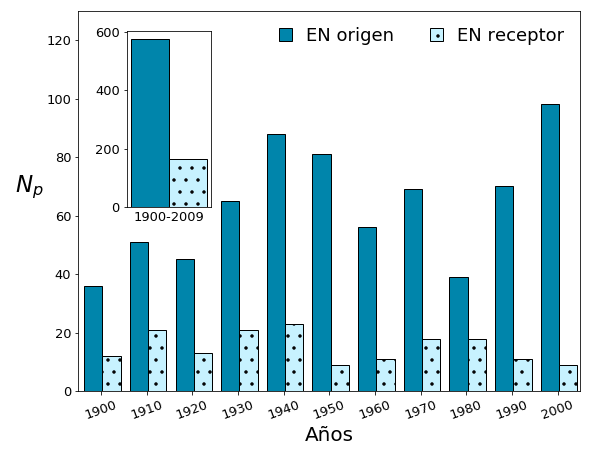
\includegraphics[width=0.5\textwidth]{BOR_EN.png} &
		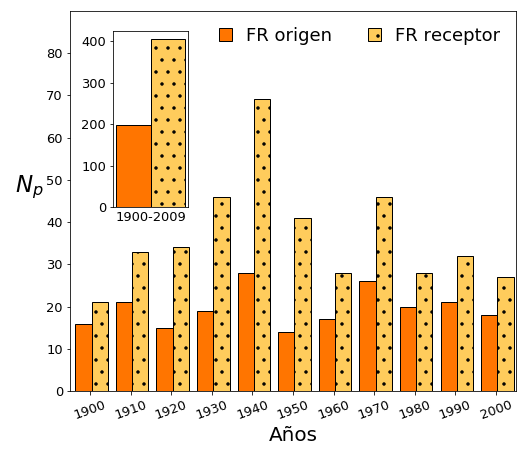
\includegraphics[width=0.5\textwidth]{BOR_FR.png} \\
		\textbf{(a)} & \textbf{(b)}   \\
	\end{tabular}

	\begin{tabular}{cc}
		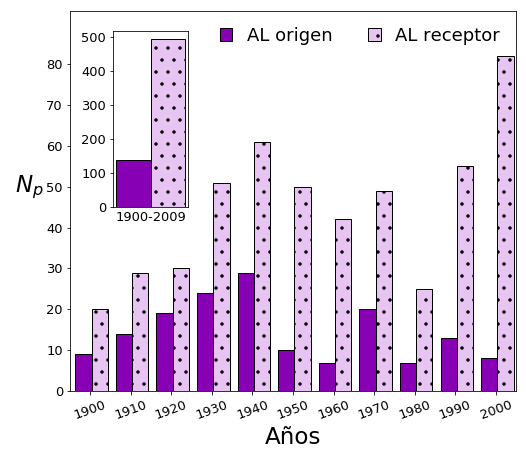
\includegraphics[width=.5\textwidth]{BOR_GE.png} &
		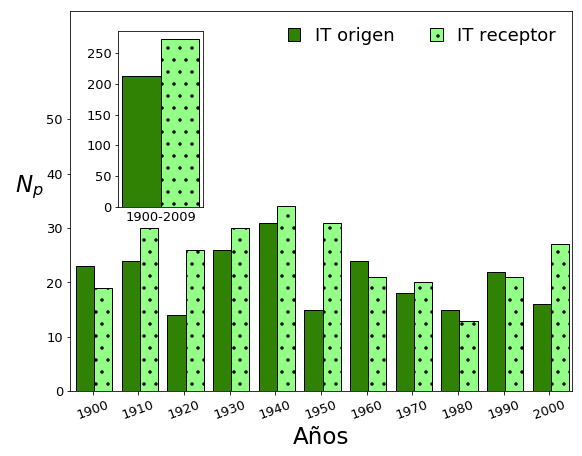
\includegraphics[width=.5\textwidth]{BOR_IT.png} \\
		\textbf{(c)}  & \textbf{(d)}   \\
	\end{tabular}
	\begin{tabular}{c}
		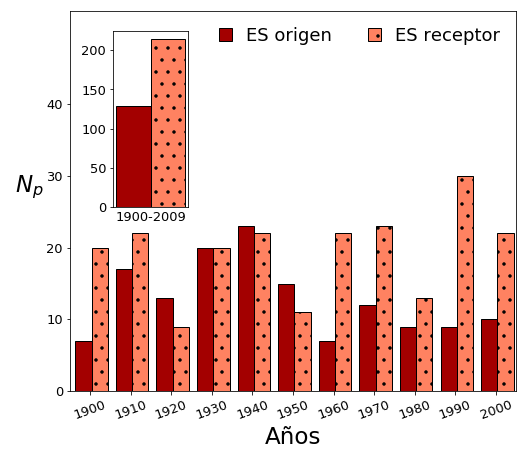
\includegraphics[width=.5\textwidth]{BOR_SP.png} \\
		\textbf{(e)} \\
	\end{tabular}
	\caption{Los idiomas como orígenes y receptores de palabras nuevas.
	Durante el siglo XX, sólo el inglés \textbf{(a)} ha sido el idioma que
	ha migrado más palabras de las que ha recibido. Francés \textbf{(b)},
	alemán \textbf{(c)}, italiano \textbf{(d)} y español \textbf{(e)}, han
	recibido más palabras durante la segunda mitad de siglo, tras finalizar
	la segunda guerra mundial. }
	\label{fig.RO_idiomas}
\end{figure} % }}}

La figura~\ref{fig.RO_idiomas} muestra el comportamiento de los idiomas al ser
orígenes o receptores de palabras nuevas.  El inglés ha aportado casi tres
veces más palabras de las que ha recibido, con sus mayores apogeos en 1940,
década que aconteció la segunda guerra mundial,  y en el 2000 tras la
globalización y el acceso a la tecnología en mayores sectores de la población. 

Francés y alemán, como receptores han sido similares, ambos recibiendo casi la
misma cantidad de palabras en cada década desde comienzos (1900) hasta mitad de
siglo (1950). Después de 1980, el alemán ha obtenido en cada década 30 palabras nuevas respecto a la década anterior, en consecuencia ha sido el mayor receptor en los últimos treinta años. Al tratarse como idioma origen, el alemán redujo la cantidad de palabras que aportaba en 1950, nuevamente tras finalizar la segunda guerra.

Referente al italiano, década a década, aporta casi la misma cantidad de
palabras que las que recibe, las únicas excepciones se dieron en 1920 y en
1950, tras finalizar la primera y segunda guerra mundial. 

Finalmente, el español en 1930 y en 1940, la cantidad de palabras que aporta y
que recibe es similar.  En las demás décadas, el español ha actuado primordial
mente como un idioma receptor. 

\subsection{Inglés} % {{{
\cpnote{aca vamos en el 3}

\begin{figure} [h!] % {{{
	\centering
	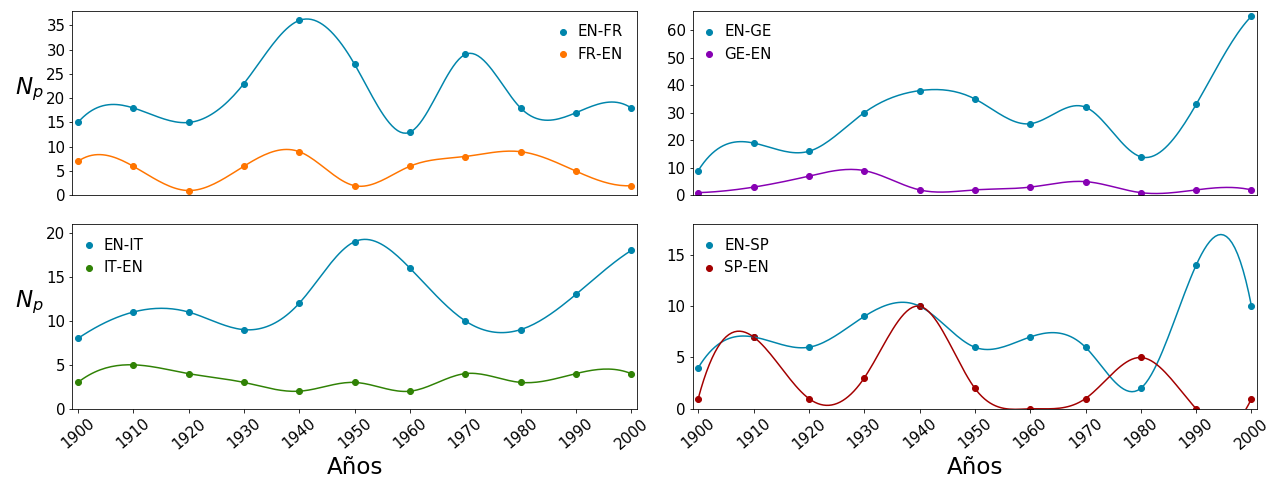
\includegraphics[scale=.33]{NC_EN.png}
	\caption{Palabras que migran del inglés a los demás idiomas y de los demás idiomas al inglés. El alemán ha sido el que más palabras recibe del inglés en promedio 29 cada década, seguido del francés con 21, el italiano con 12 y el español con 7. Los campos semánticos comunes en las migraciones del inglés a los demás idiomas son la política, la economía, la globalización y la tecnología.}
	\label{fig.NC_EN}
\end{figure} %  }}}

%De manera general, el idioma que más se ha beneficiado del inglés ha sido el alemán, con 300 préstamos en 100 años.  Inglés y alemán forman parte de las lenguas germánicas,  posible razón de los mayores intercambios. Entre las lenguas romances, el francés fue el más favorecido, pero también es la más similar por las relación normanda entre ambas.

De la figura~\ref{fig.NC_EN}, se puede ver que el inglés (con cualquier combinación) migró más palabras nuevas de las que recibió; las únicas excepciones se dieron  con el español en las décadas de 1910, 1040 y 1980. 
%A pesar de ser el mayor portador, la cantidad de palabras nuevas en los diferentes receptores no es homogénea, por ejemplo en el francés  la cantidad mínima por década es de 13, mientras que el español recibió un máximo de 14 en 1990.  Al tomarse como receptor hay más homogeneidad, ya que la media de palabras recibidas por década en cualquier combinación ronda  entre 3 y 5. 

Entre 1920 y 1950, el francés, el alemán y el italiano tuvieron un incremento de palabras del ingles. En este periodo las palabras encontradas son términos de las guerras, donde los Estados Unidos, el Reino Unido, Francia, Italia, Alemania y  el Imperio Austro-Húngaro estuvieron involucrados, a diferencia de España que no participo.   

Una tendencia similar se dio en los últimos veinte años (1980-2000), con un incremento del inglés en el alemán, el italiano y el español. El hecho con el que se relaciona el incremento es que el inglés se ha mostrado como un idioma común en la comunicación, la ciencia y la tecnología,  sumado al poder que obtuvo los Estados Unidos tras la segunda guerra mundial y donde su modelo económico prevaleció después de la guerra fría (conflicto que termino en 1990). 



\subsubsection*{Inglés-Francés} % {{{


Los mayores aportes se dieron entre 1930 y 1970, periodo que engloba comienzos de la Gran Depresión (1929), la Segunda Guerra Mundial (1939-1945) y la Guerra Fría (1945-1991), sucesos donde participaron países de ambas lenguas. Las palabras nuevas que refieren a estos eventos son \textit{churchill} (1944), \textit{territories} (1944), \textit{nazis} (1945), \textit{catastrophe} (1945), \textit{dollar} (1950), \textit{nixon} (1968) y \textit{johnson} (1970); las ultimas son apellidos de los presidentes de los Estados Unidos  Lyndon B. Johnson y Richard Nixon, cuyos periodos de gobierno fueron  entre 1963-1969 y 1969-1974 respectivamente.

% }}}
\subsubsection*{Inglés-Alemán} % {{{

Sólo  en dos décadas (1900  y 1980), el alemán no fue el idioma que más prestamos recibió  del ingles. Por el año de aparición, palabras como \textit{economic} (1929), \textit{depression} (1931), \textit{investment} (1933) y \textit{roosevelt} (1935), son del campo semántico de la economía y de la Gran Depresión,  mientras que  Franklin D. Roosevelt fue el presidente de los Estados Unidos que gobernó posterior a la crisis económica y durante la segunda guerra mundial. 

%La crisis económica de la gran depresión, originada en los Estados Unidos con consecuencias en diferentes países, entre ellos  Alemania, fue uno de los motivos que propició la segunda guerra mundial.

En las ultimas dos décadas, surgen términos referentes a la globalización y al desarrollo tecnológico, entre ellas \textit{standards} (1983), \textit{market} (1994), \textit{internet} (1996), \textit{economy} (1996), \textit{online} (1998), \textit{value} (2001), \textit{financial} (2003) y \textit{customer} (2007). 
% }}}
\subsubsection*{Inglés-Italiano} % {{{


Las palabras hacia el italiano, identificables en la primera mitad de siglo son \textit{roosevelt} (1941) y \textit{stalin} (1949), apellidos de personajes involucrados en la Segunda Guerra Mundial. En el caso de Joseph Stalin, a pesar de que su nacionalidad no es de algún país de habla inglesa, en el inglés su apellido tomó notoriedad para exportarse a los otros idiomas, siendo un ejemplo de palabras que se hacen populares en idiomas distintos al idioma origen. 

En los últimos años, nuevamente la globalización, la tecnología y la economía, son áreas comunes para los préstamos del inglés, \textit{internet} (1996), \textit{bussines} (2000) y \textit{marketing} (2001), son ejemplos de ellas. 


\subsubsection*{Inglés-Español} 

% aclarar esta justificacion
El español ha sido el idioma que menos préstamos toma del ingles,  sin  embargo es el idioma en el que migraron más apellidos de presidentes de los Estados Unidos, \textit{roosevelt} (1941), \textit{truman} (1950), \textit{kennedy} (1961), \textit{johnson} (1966),  \textit{nixon} (1972),  \textit{reagan} (1987), \textit{bush} (1990) y \textit{clinton} (1995).  Una de las posibles razones de encontrar en el español a estos personajes,  es por la relación y la mezcla cultural que han tenido los Estados Unidos con países de Latinoamérica.  

El los últimos años, las palabras aluden a términos de la globalización y la tecnología  \textit{internet} (1995), \textit{mail} (1999), \textit{marketing} (2001),  \textit{digital} (2002), \textit{software} (2004) y \textit{management} (2009).  

%A pesar de no ser el idioma más favorecido es al que en más areas ha impregnado el ingles, siendo este un factor que también puede indicar una mayor influencia,  en cuantas áreas esta presente un idioma y que tanto se utiliza. 

% }}}
% }}}
\subsection{Francés} % {{{

\begin{figure}[h!]
	\centering
	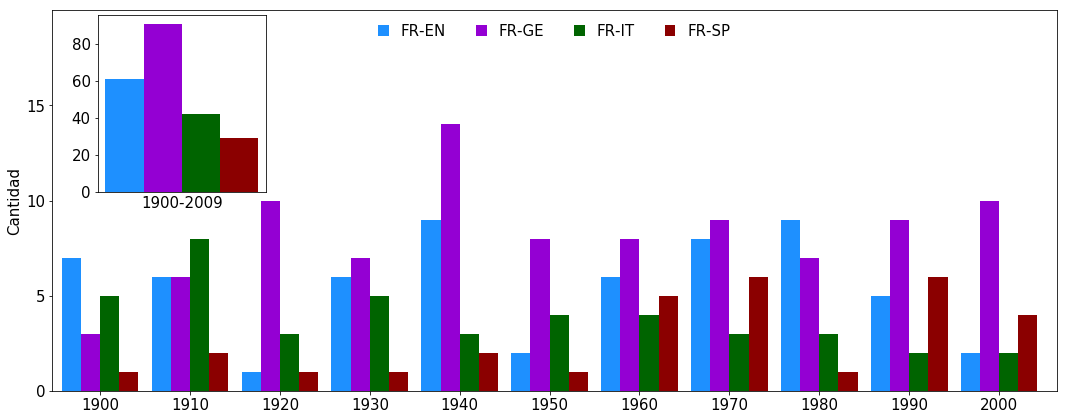
\includegraphics[scale=.33]{NC_FR.png}
	\caption{Palabras que migran del francés a los demás idiomas y de los demás idiomas al francés.  El inglés es el idioma que mas palabras recibe del francés, en promedio 8 por cada década, seguido del alemán con 5, el italiano con 3 y el español con 2. La primera y segunda guerra mundial son los campos semánticos más comunes en las migraciones del francés.}
	\label{fig.NC_FR}
	
	
\end{figure}

De la figura~\ref{fig.NC_FR} se puede ve que entre las décadas de 1920 y 1940,  incrementaron las palabras que migraron del francés en  el inglés, en el alemán y en el italiano. Las palabras que migran entre estas décadas son referentes a la Primera Guerra Mundial (que termino en 1918, año cercano a 1920) y a la Segunda Guerra Mundial (finalizada en la década de 1940). 

A pesar de que en los conflictos bélicos del siglo pasado no participaron países hispanohablantes, el español si recibió palabras que tomaron importancia tras la Segunda Guerra Mundial como lo son nombres de países y nombres de organizaciones. Este tipo de palabras son con las que se relaciona el incremento del francés en el español durante la segunda mitad de siglo. 



\subsubsection*{Francés-Inglés}% {{{

Durante el siglo XX, los préstamos en este sentido, se caracterizan por ser palabras comunes e identificables de origen inglés,  por ejemplo  \textit{diagnostic}, \textit{clients}, \textit{placement}, \textit{adaptation}, \textit{diffusion} y \textit{amplitude}.  A pesar de ser errores en los resultados, este tipo de palabras si surgieron primero en el francés, por lo que el algoritmo designó a esta lengua como el origen. 

% }}}
\subsubsection*{Francés-Alemán}% {{{

El alemán tuvo dos décadas entre 1920 y 1940  (años cercanos a las dos guerras mundiales), donde  fue el idioma que más palabras recibió del francés, entre estos años se localizaron a \textit{diplomatie} (1917), \textit{bourgeoisie} (1919), \textit{politique} (1920)  \textit{guerre} (1925), \textit{allemagne} (1925), \textit{russie} (1925) y \textit{empire} (1937), palabras del campo semántico de la política y de países involucrados en las guerras. 



% }}}
\subsubsection*{Francés-Italiano}% {{{

Las clasificaciones para esta pareja de origen y receptor son escasas, entre las pocas realizadas se encuentra un término del campo científico como \textit{poincare} (1924) (apellido del matemático francés Henri Poincaré);  y nombres de ciudades y países referentes a las dos guerras mundiales, \textit{austro} (1915), \textit{versailles} (1924), \textit{vietnam} (1966)  y \textit{urss} (1975).


% }}}
\subsubsection*{Francés-Español}% {{{


En el español, las palabras que provienen del francés son del campo semántico de la Posguerra de la Segunda Guerra Mundial, entre ellas estan nombres de países como {urss} (1962) y \textit{vietnam} (1965); y nombres de organizaciones \textit{onu} (1995) y  \textit{ocde} (2009). A pesar de que en la Organizacion de las Naciones Unidas (ONU) y en la Organización para la Cooperación y el Desarrollo Económico (OCDE) sean miembros países cuya lengua oficial no sea ni francés ni español,  en francés y español la abreviación de estas organizaciones es la misma.  

%




% }}}
% }}}
\subsection{Alemán}% {{{

\begin{figure}[h!]
	\centering
	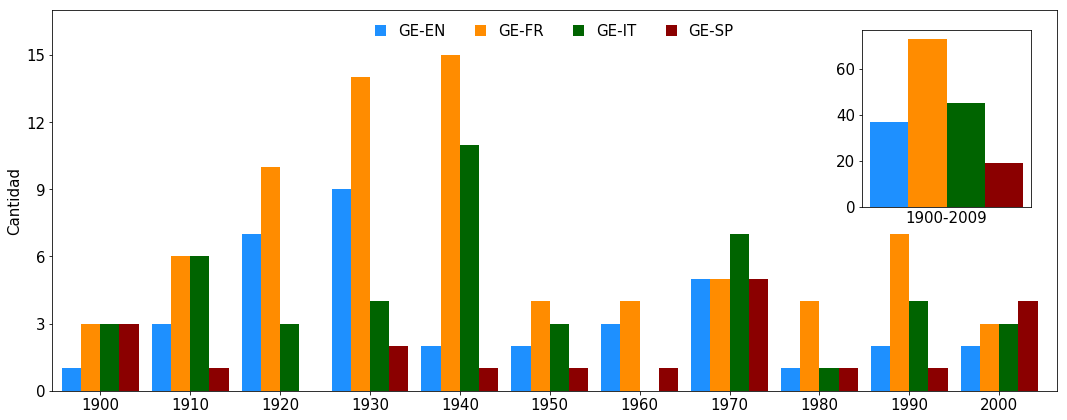
\includegraphics[scale=.33]{NC_GE.png}
	\caption{Palabras que migran del alemán a los demás idiomas y de los demás idiomas al alemán. El francés es el idioma que más palabras recibe del alemán,  en promedio 6 por cada década,  seguido del ingles y el italiano con 4,  por ultimo esta el español con 2. Los campos semánticos más comunes en las migraciones del alemán son la guerra  y  los apellidos  de personajes germano parlantes que destacaron en algún área academia.}  
	\label{fig.NC_GE}
\end{figure}



De la figura~\ref{fig.NC_GE} se puede ver que entre las décadas de 1920 y 1940, en todos los idiomas aumentaron la cantidad de palabras migraban del alemán, mientras que en la segunda mitad de siglo disminuyeron, salvo en la décadas de 1970 con el italiano y con el español, y en el 2000 con el español, resultando el alemán un idioma que recibió más palabras de las que migró,  La participación de Alemania en los conflictos bélicos, propició que las migraciones del alemán en la primera mitad de siglo surgieran del campo semántico de la guerra, mientras que la derrota de Alemania es un factor para que el alemán en la segunda mitad recibiera más palabras, adaptándose a ámbitos culturales, políticos y económicos de los demás países. 

Los personajes germano parlantes que destacaron en algún areá, con excepción de Hitler, no son identificables en la figura~\ref{fig.NC_GE}, ya que no migraron en el mismo año en que destacaron, y en cada receptor el año de migración es diferente. 


\subsubsection*{Alemán-Inglés}% {{{

En los años posteriores a la Segunda Guerra Mundial, se encontraron palabras ligadas al evento, entre ellas \textit{lenin} (1931), \textit{hitler} (1934) y \textit{reich} (1939).  Otras palabras relevantes son \textit{beethoven} (1930), \textit{marx} (1934) y \textit{freud} (1934), apellidos de personajes destacados en la música, la filosofía y la psicología, todos ellos germano parlantes.


% }}}
\subsubsection*{Alemán-Francés}% {{{

%El francés ha recibido más palabras del alemán que cualquier otro. A pesar de que la mayor cantidad de aportes se dio en la primera mitad de siglo, las relaciones que se encontraron han sido a lo largo de todo el periodo y en diferentes áreas. 

Se distinguieron dos campos comunes para los préstamos nuevos,  el primero referente a la historia del alemán en las guerras, \textit{kaiser} (1915), \textit{reich} (1921), \textit{hitler} (1933),  \textit{regierung}, \textit{deutschen},\textit{minister} y  \textit{bestimmungen} todas ellas en 1944. % (traducciones de gobierno, alemán, ministro y reglamentos).  

El segundo campo, son apellidos de  personajes destacados en la filosofía \textit{nietzsche} (1905),  \textit{marx} (1923), \textit{engels} (1970) y \textit{heidegger} (1987); la psicologia \textit{freud} (1965)  y  la música \textit{mozart} (1956). 



\subsubsection*{Alemán-Italiano}% {{{

Los préstamos que migraron del alemán al italiano,  se encuentran palabras relacionadas con la guerra  entre ellas \textit{reich} (1930),  \textit{hitler} (1939), \textit{lenin} (1944) y \textit{berchtold} (1944); mientras que 
\textit{nietzsche} (1903),  \textit{engels} (1948) y  \textit{heidegger} (1978) son de la filosofía; \textit{freud} (1970) en la psicologia; y \textit{mozart} (1942) y \textit{bach} (1949) en la música. 



%Nuevamente los préstamos del alemán,  son apellidos de personajes destacados en algun ar,  además de los ya mencionados, el único apellido exclusivo en el italiano fue \textit{berchtold} en 1943, referente a Leopold Berchtold, ministro de exteriores del Imperio Austro-Húngaro de 1912 a 1915, cuyo fallecimiento ocurrió en 1942. R


  
% }}}
\subsubsection*{Alemán-Español}% {{{

A pesar de que el español no estuvo involucrado en la segunda guerra mundial, si migrarón a él terminos relacionados con el suceso,  entre ellos \textit{kaiser} (1938) y \textit{hitler} (1940). 

Las demás palabras son nuevamente  apellidos de personajes, \textit{marx} (1932), \textit{lenin} (1970), \textit{hegel} (1971),  \textit{nietzsche} (2000) y \textit{freud} (2002). Estas palabras a pesar de ser comunes en las migraciones del alemán, la migración hacia el español ocurrió después que los demás idiomas, por ejemplo en el francés Nietzsche apareció en 1905 y Freud en 1934. La diferencia en los años de migración puede ser un indicio de la adaptabilidad de una lengua en otra, aunque en este trabajo no se ha desarrollado esta idea. 



% }}}
% }}}

% {{{

\clearpage
\subsection{Italiano}
 
 
\begin{figure}[h!]
	\centering
	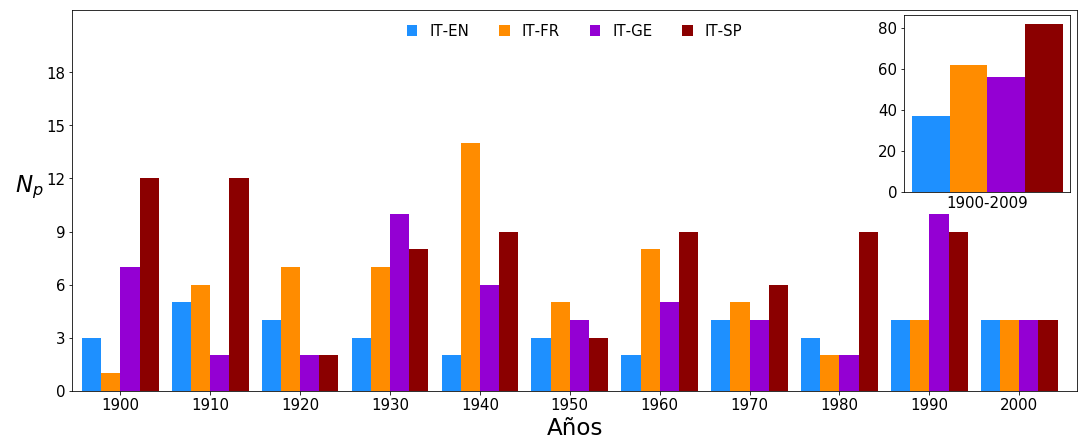
\includegraphics[scale=.33]{NC_IT.png}
	\caption{Palabras que migran del italiano a los demás idiomas y de los demás idiomas al italiano.  El español es el idioma que más palabras recibe del italiano, en promedio 8 por cada década, seguido del francés con 6,  el alemán con 4 y el inglés con 3. Los campos semánticos de la guerra y la política comunes en la migraciones del italiano .} 
	\label{fig.NC_IT}
\end{figure}



De la figura~\ref{fig.NC_IT} se observa que unicamente con el ingles, el italiano ha sido exclusivamente un idioma receptor,  con los demás idiomas,  el italiano es tanto el que más palabras migra como el que más recibe. 

Las migraciones del italiano en el alemán, en el francés y en español, aumentaron  entre 1920 y 1940,  coincidiendo este periodo con las dos guerras mundiales (La Primera Guerra mundial termino en 1918, año cercano a 1920), situaciones donde participo Italia, por lo que los préstamos son referentes a estos  sucesos. 

En todos los idiomas,  a partir de 1990, se presenta un descenso en la cantidad de palabras que llegan del italiano, posiblemente al no estar relacionado el italiano con la globalización y el desarrollo tecnológico, los sucesos más importantes  desde esa década.   

\subsubsection*{Italiano-Inglés}% {{{

A pesar de que en cada década existen términos nuevos en el inglés, sólo fue posible relacionar \textit{mussolini} (1935),  alusivo al político y militar Benito Mussolini,  posiblemente el personaje italiano más relevante en la historia del siglo XX .

% }}}
\subsubsection*{Italiano-Francés}% {{{



En las migraciones sólo se asoció \textit{mussolini} (1935), la cual ya se había mencionado. Aunque en 1940 migraron la mayor cantidad de préstamos, ninguno se logro relacionar con eventos al rededor de la década. 

Tras revisar las listas de los préstamos nuevos con origen italiano  en los demás idiomas, Mussolini se encuentra en todas ellas, donde el año de migración es siempre 1935.





% }}}
\subsubsection*{Italiano-Alemán}% {{{

En este sentido de migración,  existen relaciones con el contexto bélico,  \textit{regime} (1938), \textit{panzer} (1941), \textit{duce} (1942),  traducciones de régimen, blindado y líder.

%además de \textit{Mussolini} (1935). 



% }}}
\subsubsection*{Italiano-Español}% {{{

En el español, además de los términos de la guerra, se encontraron nombres de términos políticos y sociales que tuvieron un auge en el siglo pasado,  \textit{socialista} (1914), \textit{comunista} (1932), \textit{capitalismo} (1935), \textit{fascismo} (1937),  \textit{marxismo} (1963) y \textit{terrorismo} (1986). 

% }}}
% }}}


\subsection{Español}% {{{

\begin{figure}[h!] % {{{
	\centering
	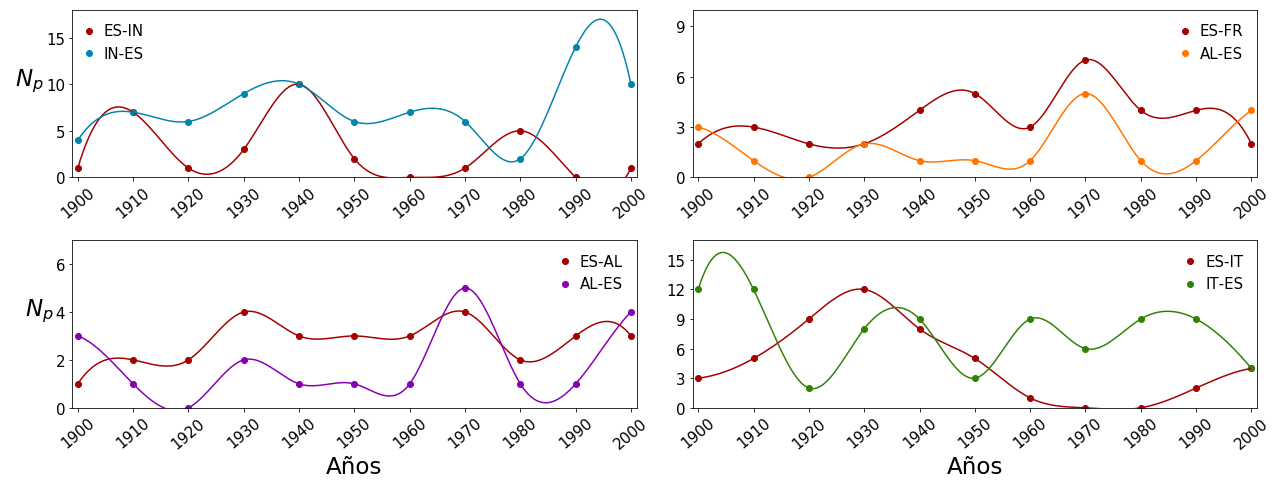
\includegraphics[scale=.33]{NC_SP.png}
	\caption{Palabras que migran del español a los demás idiomas y de los demás idiomas al español. El italiano es el idioma que más palabras recibe del español, en promedio 5 por cada década, seguido del francés con 3, mientras que el ingles y el alemán reciben 2. Los campos semánticos donde provienen los préstamos del español  más comunes en las migraciones del español son la medicina y los nombres de países y Latinoamericanos. }
	\label{fig.NC_SP}
\end{figure} % }}}


De la figura~\ref{fig.NC_SP}, se pueden ver comportamientos similares en las migraciones del español en los demás idiomas, con incrementos en la primera década del siglo y entre las décadas de 1930 y 1940,  y una disminución desde 1990. En algunos casos las migraciones fueron nulas, en el ingles en las décadas de 1960 y 1990, mientras que en el italiano fueron entre las décadas de 1970  y 1980. 

Tras revisar los pŕestamos del español en los diferentes receptores,  la característica común de los préstamos es que son términos médicos, migrando en los diferentes receptores en la primera mitad de siglo, por lo que son la principal razón de del incremento entre 1930 y 1940. 

Al igual que en el italiano, las migraciones del español en los demás idiomas (salvo en el italiano) decayeron a partir de la década de 1990, ya que el español no ha tenido relación con la globalización y el desarrollo tecnológico. 

\subsubsection*{Español-Inglés}% {{{

Contrario a la tendencia en las migraciones anteriores, la guerra no es un campo semántico común en el contenido de los préstamos. La mayor parte de los términos son habituales en la medicina,  en 1943  aparecieron  \textit{virus} y \textit{anemia};  años antes en 1934 George Richards Minot, Parry Murphy y George Hoiyt Whipple, habían recibido el premio Nobel de medicina por su descubrimiento de la terapia de hígado para el tratamiento de anemias.   

Otras pañabras importantes son nombres de países hispanohablantes \textit{chile} (1919) y \textit{argentina} (1940); de acuerdo a \cite{crisis_chile} tras la primera guerra mundial, Chile se vio en una crisis económica  que culmino hasta 1930 gracias al desarrollo de la industria fabril chilena; por otra parte a la década de 1930 también se le conoce como la década infame en la historia argentina, debido a la crisis económica que sufrió el país  y que llevo a un golpe de estado durante el mandato del presidente Hipólito Yrigoyen. 

\subsubsection*{Español-Francés}% {{{

El primer préstamo con contenido es \textit{panama} (1913), su importancia se debe a la inauguración del canal de Panamá en 1914. Destaca que la palabra llegue al francés por ser el gobierno de Francia el que impulsó económicamente su construcción, aunque su conclusión y administración pasó a los Estados Unidos.  




% }}}
\subsubsection*{Español-Alemán}


Los préstamos son nuevamente términos médicos, además \textit{virus} y \textit{anemia} mencionados en las migraciones hacia el inglés. Como termino exclusivo en el alemán  se encontró a \textit{lepra} (1901), debido a que en 1874, Gerhard Armauer Hansen descubrió el bacilo de Leprae que origina la enfermedad.

%fue globalmente importante a partir de 1874,  ya que en ese año el científico noruego Gerhard Armauer Hansen descubrió el bacilo de Hansen Mycobacterium Leprae \cite{lepra} que origina la enfermedad. Por el carácter médico de la palabra, es probable que se hiciera más investigación sobre la enfermedad en diferentes idiomas, en este caso el alemán. 


% }}}
\subsubsection*{Español-Italiano}% {{{

Además de los términos médicos ya mencionados, en el italiano migraron de forma  exclusiva  \textit{virus} (1922), \textit{colesterina} (1928),  \textit{sintomatología} (1931), \textit{anestesia} (1932), \textit{vitamina} (1935), \textit{anemia} (1936), \textit{metabolismo} (1936),  \textit{gástrica} (1936)  y \textit{endovenosa} (1937).  

También destacan las palabras  \textit{buenos} (1900) y \textit{aires} (1901), referentes a Buenos Aires, la capital de Argentina . Este préstamo esta ligado a la migración de personas,  ya que desde 1862 hasta 1970, incremento la población de italianos en Argentina,  asentándose principalmente en la ciudad de Buenos Aires,  además para 1900 los inmigrantes italianos representaban casi 20$\%$ de la población en Argentina.  Tras la inmigración de italianos en Argentina, es común pensar que esta mezcla origino cambios culturales, entre ellos en los idiomas. 

%El aparecer estas palabras en el español (dentro de las cinco mil más usadas)antes que en los demás,  sugiere que la medicina era un campo importante para los países de habla española, donde posiblemente se publicaron más libros de medicina en esta lengua. 






% }}}
% }}}
% }}}
\section{Resultados generales}% {{{



Tras las múltiples combinaciones entre idiomas, la relación habitual son palabras del campo semántico de la guerra, la mayor parte de ellas, surgieron en los diferentes receptores durante y después de la Segunda Guerra Mundial. 

En cada idioma, las migraciones de palabras son recurrentes de ciertos campos semánticos,  el inglés en economía, tecnología y política; el español en medicina, y en la cultura de los países Latinoamericanos; el francés y el italiano en la guerra; mientras que en el alemán además de la guerra también son comunes las áreas académicas  a partir de personajes germano parlantes que destacaron en ellas. .  

Las áreas mencionadas, no brindan una respuesta sobre que idioma ha sido más influyente, pero si en cuales campos un idioma ha influido más que los otros, siendo esta una forma alternativa de hablar de influencia en los idiomas.
 
Una manera diferente de estudiar a los préstamos nuevos, sería a través del tiempo que le toma a las palabras moverse de un idioma a otro, con ello, se pueden obtener la velocidad con la que migran y su adaptabilidad en las diferentes lenguas receptoras. Aunque estos resultados pueden ser complementarios, por el momento no se han tratado. 


%El inglés se presenta en las últimas dos décadas como el idioma común para transmitir información, exportando términos comunes en ámbitos como  la globalización y el desarrollo  de la tecnología.  Destaca el rol de los Estados Unidos como un país involucrado en los principales acontecimientos que originaron las migraciones, siendo usuales los apellidos de todos sus presidentes (posteriores a la segunda guerra mundial) en los demás idiomas. 

%Salvo el inglés que fue exportador en distintas áreas, los demás idiomas se caracterizaron por brindar palabras especificas,  el alemán por apellidos de personajes, el español por términos médicos, mientras que el francés y el italiano por la historia bélica y la religión. . 

 %Estos posibles resultados ayudarían a complementar la relación entre eventos, ya que en algunos eventos las palabras asociadas a él, migraron a los demás idiomas  en el mismo periodo, por ejemplo,  las palabras que migraron tras la revolución francesa (1789-1799) aparecieron en los diferentes receptores mientras ocurría el suceso y hasta veinte años después de él; así mismo,  los términos involucrados en la globalización  posterior a 1980 migraron en los años inmediatos a su invención.  Para tales complementos se necesitaría separar a los préstamos por áreas, lo cual no se hizo en este trabajo.  












% }}}



